% From https://github.com/UWIT-IAM/UWThesis
\documentclass[print]{nuthesis}
\usepackage{amssymb, amsthm, amsmath, amsfonts}
\usepackage{wasysym}
\usepackage{mathrsfs}
% \usepackage{hyperref}
\usepackage{graphicx}
\usepackage{lineno}
\usepackage[colorinlistoftodos]{todonotes}
\usepackage{listings}
%\usepackage{breqn}
\usepackage{cancel, enumerate}
\usepackage{rotating, environ}
\usepackage{caption}
\usepackage{subcaption}
\usepackage[inline]{enumitem}
\usepackage{dirtree}

\newtheorem{thm}{Theorem}
\newtheorem{defn}{Definition}
\newtheorem{prop}{Proposition}
\newtheorem{lemma}{Lemma}
\newtheorem{cor}{Corollary}

% Syntax highlighting #22
\usepackage{color}
\usepackage{fancyvrb}
\newcommand{\VerbBar}{|}
\newcommand{\VERB}{\Verb[commandchars=\\\{\}]}
\DefineVerbatimEnvironment{Highlighting}{Verbatim}{commandchars=\\\{\}}
% Add ',fontsize=\small' for more characters per line
\usepackage{framed}
\definecolor{shadecolor}{RGB}{248,248,248}
\newenvironment{Shaded}{\begin{snugshade}}{\end{snugshade}}
\newcommand{\AlertTok}[1]{\textcolor[rgb]{0.94,0.16,0.16}{#1}}
\newcommand{\AnnotationTok}[1]{\textcolor[rgb]{0.56,0.35,0.01}{\textbf{\textit{#1}}}}
\newcommand{\AttributeTok}[1]{\textcolor[rgb]{0.77,0.63,0.00}{#1}}
\newcommand{\BaseNTok}[1]{\textcolor[rgb]{0.00,0.00,0.81}{#1}}
\newcommand{\BuiltInTok}[1]{#1}
\newcommand{\CharTok}[1]{\textcolor[rgb]{0.31,0.60,0.02}{#1}}
\newcommand{\CommentTok}[1]{\textcolor[rgb]{0.56,0.35,0.01}{\textit{#1}}}
\newcommand{\CommentVarTok}[1]{\textcolor[rgb]{0.56,0.35,0.01}{\textbf{\textit{#1}}}}
\newcommand{\ConstantTok}[1]{\textcolor[rgb]{0.00,0.00,0.00}{#1}}
\newcommand{\ControlFlowTok}[1]{\textcolor[rgb]{0.13,0.29,0.53}{\textbf{#1}}}
\newcommand{\DataTypeTok}[1]{\textcolor[rgb]{0.13,0.29,0.53}{#1}}
\newcommand{\DecValTok}[1]{\textcolor[rgb]{0.00,0.00,0.81}{#1}}
\newcommand{\DocumentationTok}[1]{\textcolor[rgb]{0.56,0.35,0.01}{\textbf{\textit{#1}}}}
\newcommand{\ErrorTok}[1]{\textcolor[rgb]{0.64,0.00,0.00}{\textbf{#1}}}
\newcommand{\ExtensionTok}[1]{#1}
\newcommand{\FloatTok}[1]{\textcolor[rgb]{0.00,0.00,0.81}{#1}}
\newcommand{\FunctionTok}[1]{\textcolor[rgb]{0.00,0.00,0.00}{#1}}
\newcommand{\ImportTok}[1]{#1}
\newcommand{\InformationTok}[1]{\textcolor[rgb]{0.56,0.35,0.01}{\textbf{\textit{#1}}}}
\newcommand{\KeywordTok}[1]{\textcolor[rgb]{0.13,0.29,0.53}{\textbf{#1}}}
\newcommand{\NormalTok}[1]{#1}
\newcommand{\OperatorTok}[1]{\textcolor[rgb]{0.81,0.36,0.00}{\textbf{#1}}}
\newcommand{\OtherTok}[1]{\textcolor[rgb]{0.56,0.35,0.01}{#1}}
\newcommand{\PreprocessorTok}[1]{\textcolor[rgb]{0.56,0.35,0.01}{\textit{#1}}}
\newcommand{\RegionMarkerTok}[1]{#1}
\newcommand{\SpecialCharTok}[1]{\textcolor[rgb]{0.00,0.00,0.00}{#1}}
\newcommand{\SpecialStringTok}[1]{\textcolor[rgb]{0.31,0.60,0.02}{#1}}
\newcommand{\StringTok}[1]{\textcolor[rgb]{0.31,0.60,0.02}{#1}}
\newcommand{\VariableTok}[1]{\textcolor[rgb]{0.00,0.00,0.00}{#1}}
\newcommand{\VerbatimStringTok}[1]{\textcolor[rgb]{0.31,0.60,0.02}{#1}}
\newcommand{\WarningTok}[1]{\textcolor[rgb]{0.56,0.35,0.01}{\textbf{\textit{#1}}}}

%% https://github.com/rstudio/rmarkdown/issues/1649
\newlength{\cslhangindent}
\setlength{\cslhangindent}{1.5em}
\newenvironment{CSLReferences}[2]%
{\setlength{\parindent}{0pt}%
\everypar{\setlength{\hangindent}{\cslhangindent}}\ignorespaces}%
{\par}

% fix for pandoc 1.14
\providecommand{\tightlist}{%
  \setlength{\itemsep}{0pt}\setlength{\parskip}{0pt}}

%% something about tables, from https://github.com/ismayc/thesisdown/issues/122
\usepackage{calc}

%% for copyright symbol
\usepackage{textcomp}

%% to allow to rotate pages to landscape
\usepackage{lscape}
%% to adjust table column width
\usepackage{tabularx}

% suppress bottom page numbers on first page of each chapter
% because they overlap with text
\usepackage{etoolbox}
\patchcmd{\chapter}{plain}{empty}{}{}

%% for more attractive tables
\usepackage{booktabs}
\usepackage{longtable}


\usepackage{graphicx}


% Double spacing, if you want it.
\def\dsp{\def\baselinestretch{2.0}\large\normalsize}
% \dsp

% If the Grad. Division insists that the first paragraph of a section
% be indented (like the others), then include this line:
\usepackage{indentfirst}

%%%%%%%%%%%%%%%%%%
% If you want to use "sections" to partition your thesis
% un-comment the following:
%
% \counterwithout{section}{chapter}
% \setsecnumdepth{subsubsection}
% \def\sectionmark#1{\markboth{#1}{#1}}
% \def\subsectionmark#1{\markboth{#1}{#1}}
% \renewcommand{\thesection}{\arabic{section}}
% \renewcommand{\thesubsection}{\thesection.\arabic{subsection}}
% \makeatletter
% \let\l@subsection\l@section
% \let\l@section\l@chapter
% \makeatother

\renewcommand{\thetable}{\arabic{table}}
\renewcommand{\thefigure}{\arabic{figure}}

%%%%%%%%%%%%%%%%%%


%% Stuff from https://github.com/suchow/Dissertate

% The following line would print the thesis in a postscript font

% \usepackage{natbib}
% \def\bibpreamble{\protect\addcontentsline{toc}{chapter}{Bibliography}}

\setcounter{tocdepth}{1} % Print the chapter and sections to the toc
% controls depth of table of contents (toc): 0 = chapter, 1 = section, 2 = subsection

\usepackage{natbib}


% commands and environments needed by pandoc snippets
% extracted from the output of `pandoc -s`
%% Make R markdown code chunks work
\usepackage{array}
\usepackage{amssymb,amsmath}
\usepackage{ifxetex,ifluatex}
\ifxetex
  \usepackage{fontspec,xltxtra,xunicode}
  \defaultfontfeatures{Mapping=tex-text,Scale=MatchLowercase}
\else
  \ifluatex
    \usepackage{fontspec}
    \defaultfontfeatures{Mapping=tex-text,Scale=MatchLowercase}
  \else
    \usepackage[utf8]{inputenc}
  \fi
\fi
\usepackage{color}
\usepackage{fancyvrb}


\ifxetex
  \usepackage[setpagesize=false, % page size defined by xetex
              unicode=false, % unicode breaks when used with xetex
              xetex,
              colorlinks=true,
              linkcolor=blue]{hyperref}
\else
  \usepackage[unicode=true,
              colorlinks=true,
              linkcolor=blue]{hyperref}
\fi
\hypersetup{breaklinks=true, pdfborder={0 0 0}}
\setlength{\parindent}{20pt}
\setlength{\parskip}{6pt plus 2pt minus 1pt}
\setlength{\emergencystretch}{3em}  % prevent overfull lines
\setcounter{secnumdepth}{2} %% controls section numbering, e.g. 1 or 1.2, or 1.2.3



%  ----  Text Colors  ------------------------------------------
%
% Assign colors to writers for review
%
\newcommand{\db}[1]{{\textcolor{blue}{#1}}}
\newcommand{\svp}[1]{{\textcolor{RedOrange}{#1}}}
\newcommand{\cochaircol}[1]{{\textcolor{Green}{#1}}}
%


%  --- Code chunk font size -----------------------------------------------
% https://stackoverflow.com/questions/38323331/code-chunk-font-size-in-beamer-with-knitr-and-latexhttps://stackoverflow.com/questions/38323331/code-chunk-font-size-in-beamer-with-knitr-and-latex

%% change fontsize of R code
\let\oldShaded\Shaded
\let\endoldShaded\endShaded
\renewenvironment{Shaded}{\footnotesize\oldShaded}{\endoldShaded}

%% change fontsize of output
\let\oldverbatim\verbatim
\let\endoldverbatim\endverbatim
\renewenvironment{verbatim}{\footnotesize\oldverbatim}{\endoldverbatim}


\begin{document}
% \linenumbers{}
%% Start formatting the first few special pages
%% frontmatter is needed to set the page numbering correctly
\frontmatter
%% from thesisdown
% To pass between YAML and LaTeX the dollar signs are added by CII
\title{An investigation into how well dashboards using open-source data support statistical visual inference for naive users.}
\author{Denise Renee Bradford}
\adviser{Susan R. VanderPlas, Ph.D}
% \adviserAbstract{}
\major{Statistics}
\degreemonth{Month}
\degreeyear{Year}
% \copyrightpage
%%
%% For most people the defaults will be correct, so they are commented
%% out. To manually set these, just uncomment and make the needed
%% changes.
%% \college{Your college}
%% \city{Your City}
%%
%% For most people the following can be changed with a class
%% option. To manually set these, just uncomment the following and
%% make the needed changes.
%% \doctype{Thesis or Dissertation}
%% \degree{Your degree}
%% \degreeabbreviation{Your degree abbr.}
%%
%% Now that we know everything we need, we can generate the title page
%% itself.
%%
\maketitle


\begin{abstract}
    In the modern digital era, the exponential growth of data has forced the development and use of user-friendly tools to visualize this data, most notably dashboards. Dashboards are essential for interpreting complex datasets and supporting well-informed decision-making because they are interactive visual representation platforms. This dissertation examines how well these dashboards, in particular those that use open-source data, enable statistical visual inference for users, or ``naive users,'' who have little or no experience with data analytics.
    Due to its democratized nature, open-source data has become a significant source of information, assisting a variety of industries from public health to urban planning. Utilizing this data in dashboards can be extremely beneficial for the general public, especially for those without a thorough understanding of data interpretation. The difficulty, however, lies in creating dashboards that can not only effectively present data but also help uninformed users make accurate statistical inferences without misunderstanding.
\end{abstract}

%% Optional
\begin{copyrightpage}
\end{copyrightpage}

%% Optional
\begin{dedication}
Dedicated to\ldots{}
\end{dedication}

%%%%%%%%%%%%%%%%%%%
% Acknowledgments
%%%%%%%%%%%%%%%%%%%
\begin{acknowledgments}
Thank you to all my people!
\end{acknowledgments}
%%%%%%%%%%%%%%%%%%%

%%%%%%%%%%%%%%%%%%%
% Grant Information
%%%%%%%%%%%%%%%%%%%
% \begin{grantinfo}
%     % Add any grant info here
% \end{grantinfo}

%%%%%%%%%%%%%%%%%%%
% ToC
%%%%%%%%%%%%%%%%%%%
\tableofcontents

%%%%%%%%%%%%%%%%%%%
% List of Figures
%%%%%%%%%%%%%%%%%%%
\listoffigures
\listoftables

%%%%%%%%%%%%%%%%%%%
% Start of the document
%%%%%%%%%%%%%%%%%%%
\mainmatter


\hypertarget{unl-thesis-fields}{%
\chapter{UNL thesis fields}\label{unl-thesis-fields}}

Placeholder

\hypertarget{introduction}{%
\section{Introduction}\label{introduction}}

Our data-driven modern civilization now depends heavily on the ability to precisely evaluate and exploit huge and complex datasets, especially in small rural towns where resources are often sparse.
This dissertation aims to make big datasets more understandable and useful by utilizing three related innovations: generalized parallel coordinate plots (GPCPs), reliable ways to look at missing data, and efficient methods to elaborate on the detection of unusual trends.
Each priority area is key for improving the GPCP technique to enable thorough and accurate data analysis across various datasets.

The accuracy of data interpretation is highest when dealing directly with numerical values or one-dimensional visual representations (Spence, 1990).
That is becoming more and more impractical. The size and dimensionality of datasets are increasing.
In order to make judgments based on data, it is necessary to find methods of simplifying and consolidating datasets without sacrificing significant information.
Often, a data visualization, such as a graph or table, serves as a go-between step between raw data and an observer's decision-making process. A data visualization is the visual depiction of information.
Essentially, it is an effort to effectively communicate synthesized data pieces in a way that is easy for an observer to understand and evaluate.

For high-dimensional data, parallel coordinate plots (PCPs) are a common visualization tool whereby data points are shown as lines intersecting each axis, therefore indicating a dimension.
Conventional PCP hinders its interpretability by having clutter and overlapping lines while handling big datasets. By including methods such as axis reordering, bundling, and dimensionality reduction to solve these problems, generalized parallel coordinate plots (GPCPs) expand the conventional PCP.
These improvements in clarity and usability of PCPs by means of data pattern highlighting and visual clutter reduction help Heinrich and Weiskopf (2013), for example, present several approaches to bundle comparable trajectories in GPCPs, so minimizing overlap and improving pattern identification; Johannsen et al.~(2012) address the advantages of dynamic axis reordering to highlight different data characteristics.

Stimulus-responsive attention is typically triggered by a certain category, where an observer learns that one element of the stimulus contains valuable information about the most promising location to search for additional information in order to make an accurate judgment.
Greensmith's ``Personal Equation of Interaction'' investigates personal variations in cognitive and perceptual capacity when using sophisticated visual interfaces (Greensmith, 2016).
This theory emphasizes the need of human characteristics in understanding and classifying composite glyphs, graphical elements expressing multidimensional data.
Applied to generalized parallel coordinate plots (GPCPs), it underlines the requirement of considering individual cognitive and perceptual variances since these influence data interpretation accuracy and efficiency. Generalized parallel coordinate charts display many dimensions within a single glyph.

Overall, this dissertation addresses theoretical and practical gaps within the existing literature and offers tangible improvements to GPCP's functionality.
By enhancing the treatment of missing data, refining outlier detection, and upgrading statistical methodologies, this research aims to extend GPCP's applicability across diverse research fields, ultimately facilitating more accurate and insightful data analysis.
Through a mix of theoretical expansion, algorithm development, and practical application, the enhancements proposed herein seek to advance the field of data visualization significantly.

\hypertarget{cognition-models-and-data-visualization}{%
\section{Cognition Models and Data Visualization}\label{cognition-models-and-data-visualization}}

Data visualization professionals are impacted by advancements in cognitive science, as evidenced by multiple research studies (Healey \& Enns, 2011; Hegarty, 2011; Crapo, Waisel, Wallace \& Willemain, 2000). Additionally, cognitive scientists contribute to developing ideas about data visualization (e.g., Kosslyn, 2006; Green, Ribarsky \& Fisher, 2009; Pinker, 1990; Lewandowsky \& Spence, 1989).

However, data visualization models primarily clarify the connection between users and the display rather than describe the cognitive processes involved in response to data visualizations.

The following will present a concise overview of data visualization methods that assert the influence of the cognitive system.

This is done partly to discover patterns and demonstrate the current level of abstraction in comprehending the connection between the observer and the data. Most models that establish a connection between the observer and data in data visualization do not.

These experiments manipulate low-level visual features not explicitly incorporated into current data visualization models. Several of the theories below show the absence of a clear relationship between perception and cognition.

Data visualization models are generally abstract, process-oriented descriptions of how the user interacts with the image.
Waisal, Wallace \& Willemain (1999) put forth a data visualization theory that proposes mental models as how observers comprehend the world.
Mental models are cognitive constructs believed by some to serve as the foundation for relational reasoning, as proposed by Johnson-Laird in 1983 and further supported by Byrne and Johnson-Laird in 1989. Mental models have three essential elements: understanding, description, and validation.
The theory of data visualization proposed by Waisal and colleagues corresponds to the initial stage of a mental model, where information is encoded, and the cognitive system readies itself for further elaboration.
The model proposed by Waisal et al.~describes a series of processes that an observer must follow to synchronize their mental representation of the information in the display with the actual display.
The system takes the observer's understanding of the data as input and generates a response that can be verified.
The initial step of the Waisal et al.~model involves constructing a mental representation based on the observers' understanding of the data visualization.
Subsequently, an observer selects a certain perspective from this mental model and accurately reproduces it based on the observed graph.
To make progress, the observer needs to assess three things: 1) if the visualization accurately corresponds to the model view, 2) if the visualization is consistent with the mental model, and 3) if the view and visualization are feasible when taking external factors into account.
Once all three conditions are satisfied, the observer proceeds to the validation stage of the mental model.
If any criteria are not satisfied, the mental model is revised, and the view is derived based on the revised mental model.

The practical implications of the research are evident in the data obtained from the think-aloud technique and mouse-tracking.
These findings, as reported by Waisel et al.~(1999), indicate that viewers do utilize certain steps in the process of comprehending the data visualization.
While the sequence of stages was not easily identifiable from the observed data, the authors propose that suggesting separate steps was beneficial for isolating sub-processes and gaining a clearer grasp of the description aspect involved in constructing a mental model.
This insight can be valuable in designing more effective data visualizations that align with the cognitive processes of the viewers.

Pinker's theory (1990) states that the mind is made of a collection of separate, natural mental modules that were developed to manage particular kinds of data and activities.
This thoery offers a unique perspective on the cognitive components involved in understanding graphs at a higher level.
It includes a matching process, which utilizes a graph schema of the suitable type, a message assembly that converts visual information into conceptual information, an interrogation stage where additional information is extracted from the graph if necessary, and finally an inferential process where decisions are made or insights are generated.

Each of these four procedures involves highly intricate matters.
The conversion of visual input into a conceptually meaningful form is a complex task, yet it is encapsulated in a single step in this model.
However, this is not necessarily a drawback.
If we consider this theory as a means to effectively break down the challenge of data visualization into smaller, more manageable components, then it is beneficial to divide an overwhelmingly large problem (how individuals comprehend graphs) into more meaningful sub-problems, such as understanding how people transform visual data into meaningful information.
Pinker defines the matching process as a component of ``cognitive fit'', which Vessey and his colleagues have separately investigated as a distinct problem.

For people to understand the data, how the information is presented is important.
Traditionally, scatterplots are great for showing how two variables are related, bar graphs are great for showing a key property of multiple levels of a single variable, and histograms are great for showing univariate distributions.
Cognitive fit is accomplished when the designer creates the appropriate tool (graph) for the task and the observer comprehends the correlation between their objective and the tool (Vessey \& Galletta, 1991).
Designing a visualization for cognitive fit involves creating compatible visual representations that accurately capture the mental representation of data.

Furthermore, if we want to show that a value is higher for one observation than another, we can visually display this difference on the graph's Y-axis (Bertin, 1983).

In his groundbreaking work ``Semiology of Graphics'' (1983), Jacques Bertin laid out a theory that changed the way we think about and use graphs to show information.
Bertin said that images are not just pictures; they are important tools for communicating and analyzing data.
Bertin came up with the idea of ``retinal variables'' -- visual attributes such as position, size, color, orientation, shape, and texture -- that can be changed to store and read data.
Bertin states that good visualizations should use these visual attributes to create patterns that are hard to see from text or numbers alone.

Bertin's theory is important in the areas of cartography and statistical graphics.
Categorical, numeric, and quantitative data were the three main types of data he classified.
It was important for him to emphasize how important it was to choose the right visual attributes based on the data and the message of the graphic.

Attaining optimal cognitive fit minimizes the cognitive load on the observer when carrying out the current task.
The cognitive fit concept is grounded in the theory of information processing (Newell \& Simon, 1972) and the recognition that individuals balance error and effort when carrying out tasks (Beach \& Mitchell, 1978; Payne, 1982; Vessey, 1994; Wickelgren, 1977).
Cognitive fit is one of several models that are based on an information processing framework.
Pinker identifies as the matching process is encompassed by ``cognitive fit'', explored by Vessey and colleagues as its own discrete problem.

Models of data visualization that make explicit the generation of the visualization (the data to the graphic stage) and the perception of the data (the graphic to the viewer) are helpful in thinking about a scientific framework for data visualization.
There are two high-level cognitive viewpoints at play: the creator and the viewer.
Wijk's model (2005) is an example of how the connection between components can be nicely explained in an information-processing manner.
The system (comprised of the data and the viewer) changes as a function of operations applied between data (input) and graphics (output).
Knowledge is updated in response to information extracted from the image, where the amount of information depends on the cognitive and perceptual properties of the observer.
van Wijk's model captures initial parts of cognitive psychology as one of three stages for environmental information extraction.

The simple model skips over a lot of interesting details, but it does so in a useful way.
To see the big picture, you have to zoom out and look at the big picture links between data and people.
Otherwise, you won't be able to make real progress toward its parts. Taking into account both the person and the data as a whole system pushes theory to accurately show how the two parts relate to each other.

Both the force-directed edge bundling (FDEB) technique and the Knowledge-Assisted Visualization and Guidance (KAVA) model enlarge the visualization capacity, as suggested by van Wijk.
By combining explicit knowledge bases and automated analytical tools, the KAVA paradigm improves visual analytics and enables more accurate and informed representations across many applications.
Conversely, FDEB bundles edges using a self-organizing technique that represents edges as flexible springs, reducing visual clutter in node-link diagrams and revealing high-level patterns without needing hierarchical structures.
van Wijk's simplified approach was less suited to efficiently handle complicated, high-dimensional data since it mostly concentrated on basic data display features without such advanced integrations.

It's helpful to think about information processors hierarchically to understand the links between data, visualization, people, and choices.
Wijk's model is very high-level and talks about the whole system. On the other hand, a lower-level information processing model can describe the mental steps a user needs to take to understand a data visualization.
In their model, Simkin and Hastie (1987) say that basic processes (similar to cognitive fit) happen between what the viewer sees and how well they understand the job.
While Pinker develops this into a more complex theory, considering extra cognitive processes and proposing a disciplined model for graph comprehension, Simkin and Hastie offer the first exploration of the cognitive phases involved. Pinker's work is thus an extension and elaboration of the fundamental ideas presented by Simkin and Hastie, so offering a better knowledge of how graphical information is handled and interpreted by users.
These basic processes are recognition, scanning, projection, and superimposition. Another thing that is important for making sense of a graph is grounding.

Researchers have found that visual anchoring changes how people see a stimulus when they are comparing (Johnson \& Pashler, 1990) or mentally rotating things (Xu \& Franconeri, 2015).
Anchoring is a process that is only talked about in theories of data visualization, but it is also a key part of other kinds of cognitive tasks (Couclelis, Gollegdge, Gale \& Tobler, 1987; Pylyshyn, 1999), which shows that it is at least a basic part of how people think.
This kind of process is very interesting because it helps make sense of data visualizations and learning more about it can improve the way we think in general.

A more standard model of information processing with input, memory, and output (Neisser, 1967) is changed to fit the task of making a choice based on a data visualization (Patterson, Blaha, Georges, Grinstein, Liggett, Kaveney, Sheldon, Havig, \& Moore, 2014).
The authors were smart to include a process that captures attention and clarifies output. It is the first form of data visualization that lets bottom-up processes change how people understand graphs independently.
In their model, the stimulus serves as the input, with encoding being the first step.
Once encoded, the information can be modified in both long-term and working memory.
Working memory and pattern recognition can alter long-term memory and influence the storage process. Together, working memory and pattern recognition collaborate to make decisions, guiding subsequent reactions.

It's helpful to think about information processors hierarchically to understand the links between data, visualization, people, and choices. Wijk's model is very high-level and talks about the whole system.
On the other hand, a lower-level information processing model can describe the mental steps a user needs to take to understand a data visualization.
In their model, Simkin and Hastie (1987) say that basic processes (similar to cognitive fit) happen between what the viewer sees and how well they understand the job.
Simkin and Hastie present the initial investigation of the cognitive phases involved while Pinker extends this into a more complicated theory considering extra cognitive processes and suggests a disciplined model for graph understanding.
Pinker's work thus serves as an extension and elaboration of Simkin and Hastie's basic principles, so providing a greater grasp of how graphical information is processed and perceived by users.
These fundamental procedures are recognition, scanning, projection, and superimposition.
Grounding is still another crucial component for understanding a graph.
This model shows the main groups of processes that need to be known to create a science of data visualization. Still, it doesn't go into detail about the different parts that are important in making the stimulus (in this case, the data visualization).

In the models we've already talked about, visual information comes in the form of a graph or plot, which is then stored in memory to consolidate into long-term memory.
In previous basic cognition research, changes to the visual world were studied independently to see how they affected simpler tasks. Key models and theories as discussed earlier in Pinker's cognitive model, which distinguishes top-down and bottom-up processes in visual comprehension and stresses the integration of mental representations with current knowledge, build the foundations of basic vision research in cognitive psychology (Pinker, 1990; Hegarty, 2011).
Introduced by Wertheimer, gestalt ideas draw attention to systems of perceptual organization including figure-ground separation (Spillmann, 2012).
Furthermore underlined by information theory post-WWII, research on attention mechanisms highlights the part of signal detection and cognitive control in visual perception (Swets, 1964; Posner, 2004).
By merging theoretical models with actual research, these essential books together progress our knowledge of visual cognition.
New research in how we understand data visualization builds on the strong base that basic vision research has laid.

Many things in the world need to be processed carefully, but this study shows that some visual details can be processed without paying full attention. ``Pre-attentive'' processing is the faster, more automatic processing of the visual environment.
Research shows that it takes less than 200 milliseconds (\textless{} 200ms) of preattentive processing to allow quick, parallel detection of core visual characteristics including color, orientation, and size without deliberate attention.
Introduced by Treisman and Gelade in 1980, Feature Integration Theory (FIT) provides that while individual features are handled preattentively, integrating them into an overall object requires focused attention, so explaining why conjunction searches---identifying goals based on multiple features---are slower and indicate for a serial search approach.
This approach emphasizes the part attention plays in binding several preattentive elements into a single perceptual experience (Mokeichev, Segev, \& Ben-Shahar, 2010; Treisman \& Gelade, 1980; Wolfe, 2021).
In contrast ``attentive'' processing is the slower, more conscious processing of a part of the visual environment.
So, making visualizations that support pre-attentive processing should free up the viewer's brain resources so they can be used more effectively in figuring out what the data means (Healey, Booth \& Enns, 1995), which will lead to a better way of sharing data.

In a survey conducted of basic research in attention, Healey and Enns (2011) identified clusters of tasks that are supported by pre-attentive processing: target detection; finding a goal-relevant unique item in an array, boundary detection; identifying distinct spatially organized, texture-based groups based upon how they differ from each other, region tracking; multiple object tracking and counting.
These findings clearly provide an evidence-based manner for making design decisions when generating data visualizations.
Suppose the goal of the creator is to show the difference between groups on two different variables, for example.
In that case, the creator may use a set of features, like color hues or blending, that allows a viewer to pre-attentively discern boundaries between the two groups on a scatter plot (Callaghan, 1990).

\hypertarget{exploratory-data-analysis-eda}{%
\section{Exploratory Data Analysis (EDA)}\label{exploratory-data-analysis-eda}}

John Tukey, in the 1970s, introduced exploratory data analysis (EDA) as a more flexible approach to statistics.
The concept places significant emphasis on utilizing visual tools to identify patterns and abnormalities in data before engaging in formal modeling.
The use of visual aids can be critical for comprehending data (Tukey, 1977).
Some methods that can be used to demonstrate the concept are box plots, histograms, and Q-Q graphs.

Advancements in computer performance allowed the creation of models that were both more complex and dynamic.
Tukey's Principles of Exploratory Data Analysis (EDA) underline the need of knowing data by means of exploration prior to the application of formal statistical techniques.
These ideas center on the idea that research should come first so that scientists could find fundamental structures and patterns. Visual analysis is essential because graphic representations enable one to spot trends, anomalies, and deviations.
Methods must be flexible to fit the specifics of the data rather than strictly following predetermined models; techniques should be resistant to departures from assumptions, such as outliers.
Simplicity is also important; using simple resources and techniques that support understanding without needless complication helps to Considered as a process that is iterative, EDA promotes the modification of first ideas and studies.
Comparative analysis is important to grasp variances and commonalities among several data subsets; data transformations should be taken into account to simplify relationships and expose more significant patterns.
Lastly, striking the right balance between quantitative analysis and qualitative insights provides an overall knowledge of the information.
Tukey's Principles of EDA are one of the most basic and extensively utilized frameworks for statistical analysis.
By stressing the significance of visual exploration, data characterization, and model evaluation, Tukey's work has helped data professionals comprehend complex data sets and make educated decisions.
In quantitative data analysis, Tukey's Principles have become the de facto norm and have significantly altered our perspective on data.

The relationship between the signifier and the signified is a fundamental principle in semiotics. Semiotics, as defined by Barthes (1972), is the examination of the correlation between a visual element (signifier) and its associated meaning or concept (signified).
Another key concept in semiotics is using syntax and semantics to express meaning effectively through visual communication.
The term ``graphic composition'' pertains to the organization and importance of the visual components of a graphic (Bertin, 1983).

Theories regarding visual representation include graphical theory (Cleveland \& McGill, 1984), preattentive processing (Treisman \& Gelade, 1980), gestalt principles (Wertheimer, 1928), and graphical brilliance (Tufte, 2001).
At the same time as he criticized typical procedures that result in misleading data representations, Tufte underlined the significance of clean, clutter-free visuals that show data accurately and efficiently.

Recent research suggests that using position and length to encode data visualization is the most effective since these visual cues fit human perceptual strengths rather perfectly.
In comparison to those employing angles, areas, or colors, research indicates that visual representations leveraging the location on a common scale and length enable more precise and efficient data interpretation.
Bar charts, for example, tend to be selected over pie charts since they reduce mistakes in quantitative comparisons via the use of length along a common axis.

Human perceptual capacities assist in emphasizing the need of lowering cognitive load and increasing decision-making accuracy by means of data visualization best practices.
In disciplines including monitoring, data analysis, and scientific research---where exact data interpretation is important---effective visualizations are essential.
Blending these ideas ensures that complicated material is clearly and effectively presented to multiple audiences, which improves the value and impact of visual data presentations.

The basic work of Cleveland and McGill significantly influenced Hadley Wickham's \texttt{ggplot2}.
Research by Cleveland and McGill in the 1980s emphasized the importance of graphical perception, particularly in regards of human decoding of quantitative data from visual representations.
Their research---including ``Graphical Perception: Theory, Experimentation, and Application to the Development of Graphical Methods''---established ideas including the need of appropriate visual encodings (Cleveland \& McGill, 1984).
These ideas support the clear and simple construction of ggplot2 visualizations.

The comprehensive framework Leland Wilkinson's ``The Grammar of Graphics'' provided for analyzing the elements of statistical graphics directly informed the design of \texttt{ggplot2}.
Highlighting the separation of data and visual representation, which Wickham embraced in \texttt{ggplot2}, Wilkinson's grammar presented an established approach for describe and build graphics (Wilkinson, 2005).
This grammar-based approach lets \texttt{ggplot2} be highly flexible and explicit, therefore allowing users to methodically create complex representations.

An important part of the Grammar of Graphics is the layered approach to plot construction, in which the visualization is built by defining distinct components (such as scales and coordinate systems).
Research by Wilkinson on perceptual concepts, such as the significance of position and length in properly communicating information (Wickham, 2010), has impacted this method.

Similarly, Michael L. Waskom's \texttt{seaborn} package was greatly inspired by Hadley Wickham's \texttt{ggplot2} work, grounded on Leland Wilkinson's ``Grammar of Graphics''.
\texttt{seaborn} uses \texttt{ggplot2}'s ideas, which include the usage of a grammar of graphics, sensible default aesthetics, and layered graphics to help create intricate, visually appealing statistical visualizations.
Waskom notes the inspirations in his work and emphasizes the importance of Wickham's contributions to modern data visualization tools, especially in terms of structured, high-level interfaces for Python plot generation (Waskom, M. L., 2021).

Additionally Michael L. Waskom's paper describes, the \texttt{seaborn} package's interface component provides a high-level, user-friendly API meant to isolate the complexity of \texttt{matplotlib} so simplifying the production of statistical visuals.
For relational graphs (\texttt{scatterplot}, \texttt{lineplot}), categorical plots (\texttt{boxplot}, \texttt{violinplot}), distribution plots (\texttt{distplot}, \texttt{kdeplot}), and matrix charts (\texttt{heatmap}, \texttt{clustermap}).
These features are designed to easily interact with data frames, manage data transformations, and apply statistical estimations straight-forwardly, so producing aesthetically pleasing graphs with little required customizing.

\begin{center}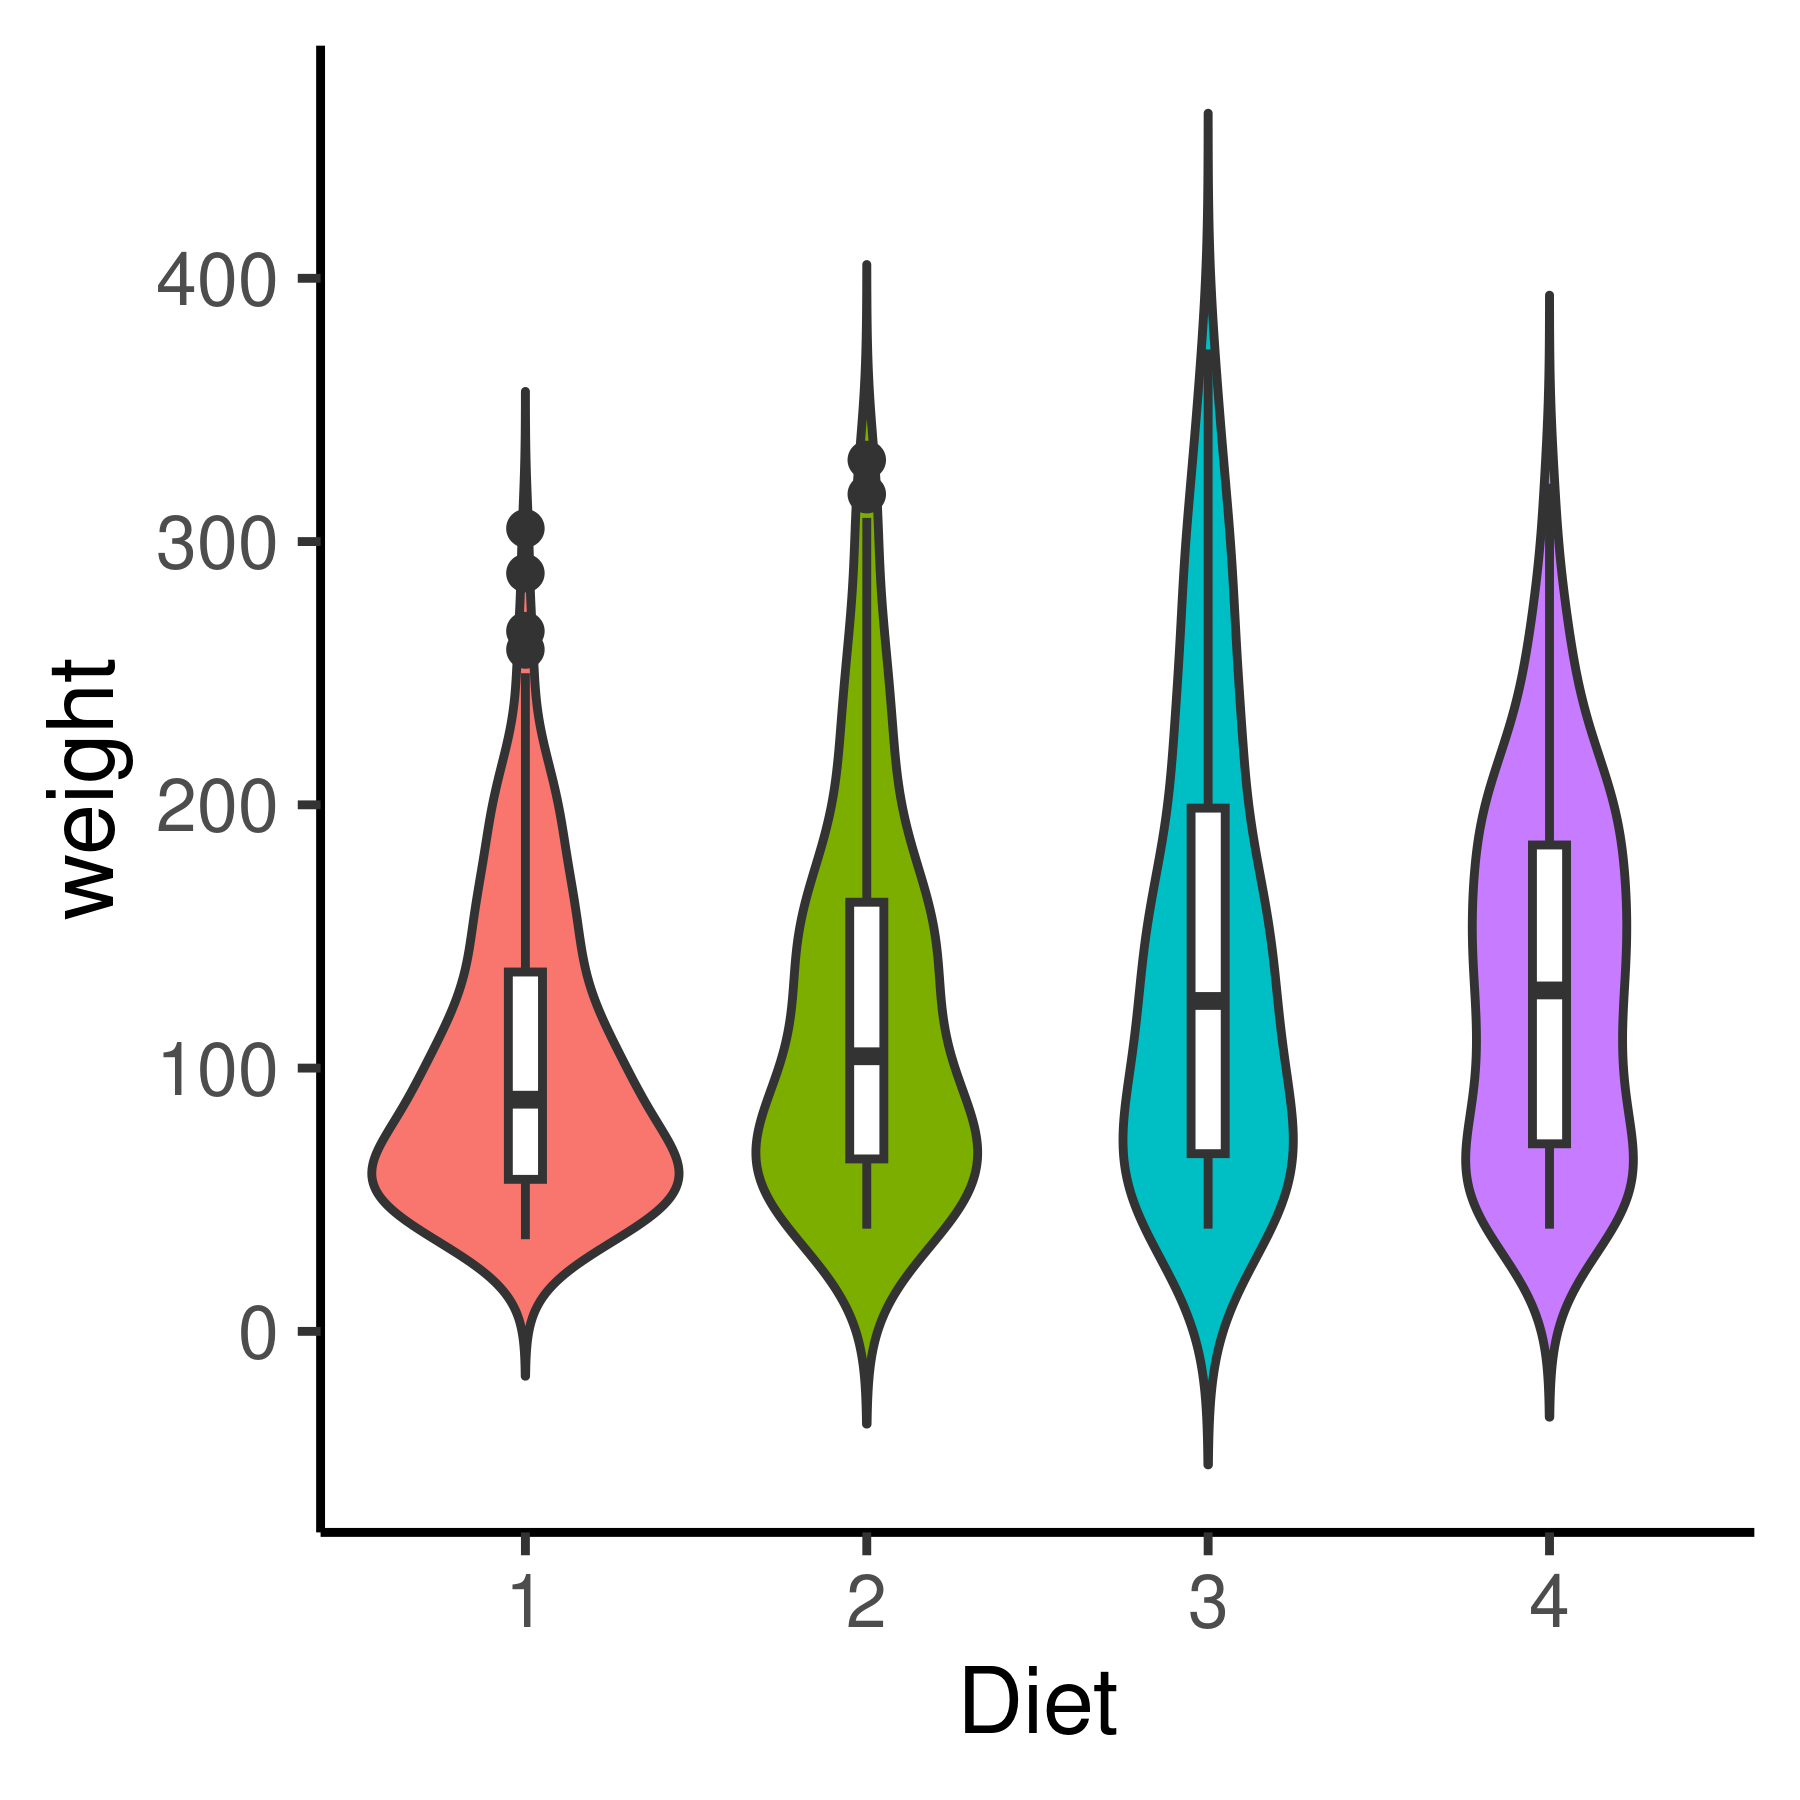
\includegraphics[width=.49\linewidth]{thesis_files/figure-latex/violin_plot-1} \end{center}

\begin{center}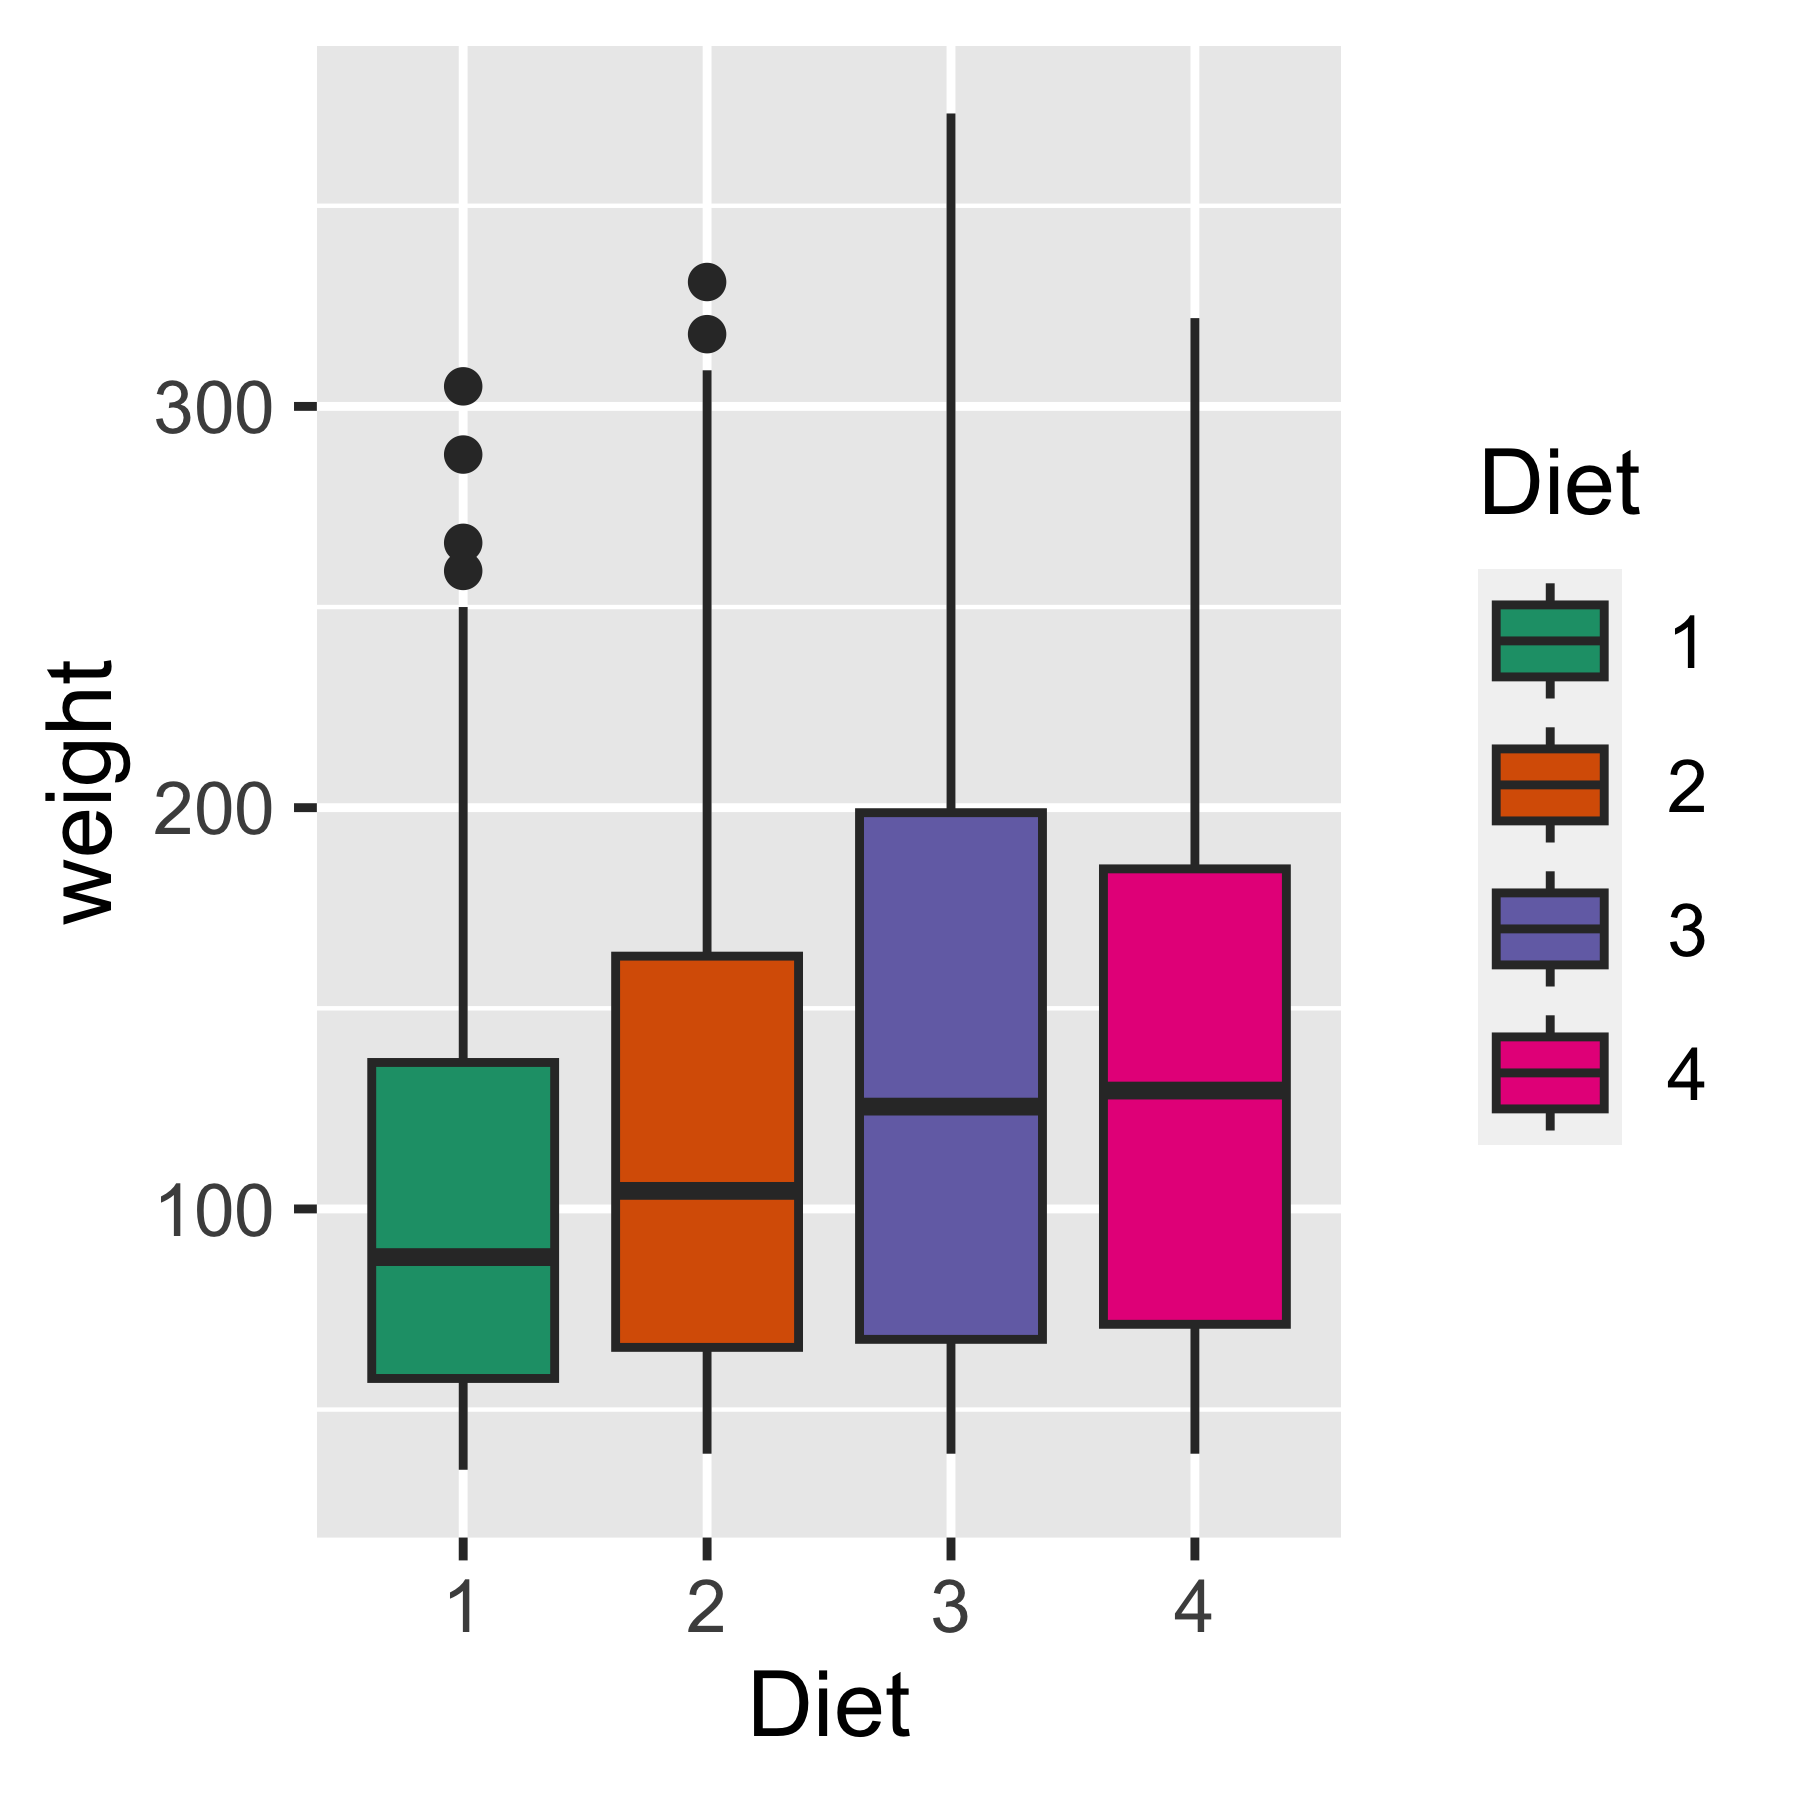
\includegraphics[width=.49\linewidth]{thesis_files/figure-latex/violin_plot-2} \end{center}

\hypertarget{parallel-coordinate-plots}{%
\section{Parallel Coordinate Plots}\label{parallel-coordinate-plots}}

Parallel coordinate plots (PCPs) are a good way to show data with a lot of dimensions, since each dimension is shown on its own plane.
This means that complex relationships between different factors can be studied over and over again.
PCPs are great for drawing attention to trends, clusters, and outliers, and they know how to use space well to show many aspects in a small area.
But because they overplot, they can get messy with large datasets.
It can be tougher to understand the data than with Cartesian coordinates, and you must go through a learning process to get the the majority of them as well.

Cartesian coordinates, on the other hand, are straightforward to understand because they are simple and well-known.
They make it easier to tell the difference between different information points and their exact values by displaying data points in an easily understood manner.
Cartesian coordinates are an excellent method to present data in a clear way because they can handle up to three dimensions.
They also have trouble with growth because adding more dimensions requires a lot of subplots or complicated three-dimensional plots, which can get boring and challenging to follow.
Cartesian graphs additionally have the ability to take up a lot of room, and for data with more dimensions, they usually need more than one plot.

If you compare PCPs to Cartesian coordinates, PCPs are a powerful way to see and analyze high-dimensional data.
However, they can cause visual clutter and require more practice to understand.
On the other hand, Cartesian coordinates are easy to understand and use for low-dimensional data but can't be scaled up or down for higher dimensions.
The data points are shown as polylines that cross the axes where their coordinate values in each part are equal (Inselberg, 1985).
Traditional parallel coordinate plots (PCPs) have helped show multidimensional data, but when the information gets more significant, they become cluttered and hard to understand.
Other versions of PCPs have been implemented in the theory to enhance the visualization and interpretation of multi-dimensional data, addressing issues such as overlap, scaling, and interaction.

In the article ``Parallel Coordinate and Parallel Coordinate Density Plots,'' Rida E. Moustafa explains a new way to see high-dimensional data using parallel coordinate plots (PCPs) and parallel coordinate density plots (PCDPs).
The primary objective of this work is to make PCPs easier to understand and use since they usually need help with too much mapping and clutter when working with big datasets.
As part of Moustafa's methodology, the standard PCP is mutated into a density plot.
This creates plot areas with more observations that stand out and reduce visual clutter.

The new approach uses density estimation methods to transform the PCP image based on polylines into a continuous, smooth depiction of data density.
This change shows how to see groups and trends usually hidden in regular PCPs.
To make things even better, Moustafa has interactive parts that let users experience different data dimensions in real time.
This makes PCPs even better at analysis. With its interactive nature, people who aren't experts can use this method confidently and successfully.

Moustafa's research indicates that to deal with even larger datasets more efficiently, future efforts should focus on enhancing density estimation methods.
These methods can be used in biology and finance to demonstrate their usefulness and adaptability for examining real-world data (Moustafa, 2011).

The article ``Orientation-Enhanced Parallel Coordinate Plots'' by Raidou et al.~describes a new way to make parallel coordinate plots (PCPs) more accessible to read and understand.
The authors suggest a method that uses input about direction to solve the clutter and overlap problems with regular PCPs.
This method changes the direction of the plot axes on the fly by applying both automatic orientation and user-interactive adjustments.
This method reduces visual noise and makes data patterns and correlations more visible.
This will make it easier for users to study and analyze large datasets.

The suggested orientation-enhanced PCPs are designed with the user's needs at the forefront, offering a more informative visual representation.
Several preprocessing steps, including principal component analysis (PCA) and multi-dimensional scaling (MDS), were employed to determine the optimal axis orientation.
This ensures that data clusters are maximally separated and data lines are minimally overlapped.
The interactive features allow users to adjust the orientation according to their preferences and requirements, enhancing the usability and adaptability of the plots for research needs (Raidou et al., 2015).

The Generalized Parallel Coordinate Plot (GPCP) is an enhancement of the original PCP that adds nonlinear axis changes.
These can show more complicated relationships in the data that might not be visible in a regular PCP.
Nonlinear scales such as logarithmic and exponential transformations are possible.
The 1997 publication ``Visualizing High-Dimensional Structures by Generalized Parallel Coordinate Plots'' by Edward Wegman and Qiang Luo provided a comprehensive discussion of the GPCP idea.
This adjustment allows the visualization to display various data connections and handle skewed data distributions.
It is important to make decisions when resources are limited, and these advanced visual tools make it easier to see how different data sets are related.
As VanderPlas et al.~(2023) show, the basic ideas put forward by Inselberg (1985) are used to build on the rules of today's graphic grammar.

\hypertarget{missing-data-analysis}{%
\section{Missing Data Analysis}\label{missing-data-analysis}}

There have been efforts to understand and deal with missing data.
Cheng et al.~(2015) made a graphical user interface for exploring missing values in multivariable data, and Josse and Husson (2016) created the \texttt{missMDA} package to handle missing values in multivariate analysis.
Since dataset incompleteness directly affects the truth of any later studies, these tools make it clear how important it is to use advanced methods to analyze and deal with it.
These methods are tailored to preserve the multidimensional relationships inherent in GPCP.

There are still issues with handling and displaying missing data in large, difficult datasets, even with the current tools and techniques.
Research has shown several approaches to handling and displaying missing data.
However, there is still a big hole in combining these methods into one system that works for all kinds of data and is easy for people to use.
Unwin et al.~showed MANET, a system that made datasets with missing values accessible through images.
Statistically speaking, lost data needs to be dealt with more complexly with even more advanced tools.
Nevertheless, the tidy data structure must be discussed in more detail.

Stef van Buuren's additional research on missing data created the \texttt{mice} package in R, which is widely used for multiple imputation.
It shows how missing data imputation methods can be used in real life, but at first, they didn't directly connect with the tidy data principles.
This gap highlights the need for a systematic strategy that combines tidy data principles with techniques for managing missing data
As a result, Tierney and Cook developed these principles to address this requirement directly.

Tierney and Cook's 2018 research expands on the principles of tidy data to create an innovative way to deal with missing data.
This method, which describes the role of missing values in data analysis and visualization, represents a major advancement in the discipline.
The paper presents valuable tools for evaluating different interpolation approaches.
These tools are critical for understanding the influence of missing data on research and the many types of imputations that may be used.
Additionally, the study offers tools that can be utilized to compare various estimation methodologies.
Because these tools are intrinsic to the R environment, you can utilize R's statistical capabilities to investigate many types of data loss.
Tools are available to help with missing data visualization, comparing imputation and non-imputed data distributions, and learning how various imputation processes impact statistical results.
Researchers will find this compilation helpful since it explains how to select the most appropriate interpolation algorithms for their data and study.

Newcomers to statistics or researchers with little to no R knowledge may need help with the approaches and code.
The dependence on R as the primary program makes the proposed approaches less accessible to those who use other statistical tools, perhaps restricting their use.

There are several opportunities for expanding their findings.
The key method for making the methodologies more accessible is to include support for other widely used data science tools in the toolkit, such as Python.
A more practical use for these tools would be an automated tool that scores and assesses various estimating algorithms using user-defined criteria.
Finally, clear instructions and examples would be useful for individuals unfamiliar with complicated data imputation techniques and tidy data architecture.

As datasets become larger and more complex, especially in fields that require visualizing high-dimensional data like genomics or big data analytics, current methods often struggle to handle the increased scale or lack the necessary flexibility to effectively address different ways in which data can be missing (Swayne \& Buja, 1998; Schafer \& Graham, 2002).
In academic study, the current state of big data analytics is centered around effectively managing large volumes, wide diversity, and fast data pace.
This poses distinct difficulties in different sectors, such as healthcare and industrial processing.
Significantly, these industries increasingly depend on advanced machine-learning methods to enhance results and prediction capacities.
Integrating big data with artificial intelligence in healthcare improves the capacity to forecast disease trends and treatment results by utilizing extensive data from various sources.
Big data analytics is vital in predictive maintenance and optimizing production processes in industrial environments.
Recent academic reviews emphasize that the future of big data analytics relies on advancing data processing technologies and ensuring their accessibility and effectiveness across various domains.
This underscores the importance of ongoing interdisciplinary research and collaboration to overcome existing barriers and unlock new opportunities (Sabharawal \& Micah, 2021; Rhaul et al., 2023).

Another common approach to present various data types is in parallel coordinates, discussed in the article ``Where Did My Lines Go?''Visualizing Missing Data in Parallel Coordinates'' by Alex Bäuerle et al.~
It is hard to see trends when data is missing because it breaks up the flow of lines. Getting rid of imputations, common ways to deal with missing data, can mess up visual presentations. Based imputation is one of many visualization methods suggested by the authors.
It keeps the general structure and doesn't lead to wrong conclusions.
Some others are dashing, imputation representation with visual cues, and transparency. Real-life studies with users showed that the best ways to find trends were to be open and dash.
The authors also made a tool that lets you use these ways to explore data more interactively. Thanks to their work, we can see incomplete information in a way that is easy to understand.
This is helpful because it avoids adding bias through estimation.
The future work includes making these methods work better with bigger datasets, mixing them with more advanced imputation techniques, and looking into how they can be used in specific fields to make them more reliable and effective (Bäuerle et al., 2022).

Addressing missing data is an analytical challenge in statistical analysis, as incomplete data can lead to biased or misleading results. These methodologies enhance data analysis and decision-making processes.
This dissertation examines advanced techniques for handling missing data, drawing from robust methodologies discussed in recent literature such as Cheng, Cook, and Hofmann (2015) and Tierney and Cook (2018).

These foundational ideas laid the groundwork for contemporary methods of handling missing data in statistical graphics, which are fundamental for providing accurate and meaningful visual interpretations of datasets.

\hypertarget{anomaly-detection-outlier-detection}{%
\section{Anomaly Detection (Outlier Detection)}\label{anomaly-detection-outlier-detection}}

In EDA, treating missing data is not merely a preliminary step but a critical anomaly detection component.
Recognizing patterns of missingness can be a powerful anomaly detection technique, as certain types of missing data may indicate underlying problems or anomalies within the dataset (Rubin, 1976).
Transitioning into anomaly detection, it becomes evident that these missing data patterns can reveal deviations from expected behavior, helping to flag data quality issues or potential outliers that warrant closer examination (Hawkins, 1980).
Thus, the systematic handling and analysis of missing data directly enrich detecting anomalies, underscoring its dual role in EDA.

Wilkinson's ``The Grammar of Graphics'' (2005) is a foundational framework for designing insightful data visualizations integral to EDA.
In this framework, treating missing data is not merely a preliminary step but a key aspect of the analytical process.
Techniques for handling missing data, such as predictive mean matching or multiple imputation, are useful for maintaining the integrity and representativeness of visualizations, allowing for more accurate interpretations and conclusions (van Buuren, 2012).

Furthermore, missing data itself can be indicative of underlying anomalies.
Analyzing patterns of missingness can reveal data integrity issues, systematic errors, or anomalies in data collection processes, which are often critical for domains like clinical trials or quality control in manufacturing (Little \& Rubin, 2002).
Once a dataset has been adjusted for missing values, visual techniques---such as enhanced scatterplots or layered density plots---can effectively detect outliers and unusual patterns.
These visualizations are pivotal in fraud detection or environmental monitoring, where quick identification of deviations from expected patterns can lead to prompt and necessary actions (Unwin et al., 2006).

Thus, handling missing data effectively enriches the dataset, enabling more robust anomaly detection through sophisticated visual tools.
This ensures that the visualizations represent the observed data and highlight the absence of data as potential markers of critical anomalies, thereby supporting deeper and more comprehensive analytical insights.

Both reducing the value of anomalies and eliminating them are primary goals of anomaly detection along with identifying their underlying cause.
Walter A. Shewhart's research on statistical control mechanisms in the 1920s is the ancestor of anomaly identification in statistical graphics.
Statistical process control (SPC) was made possible by Shewhart's creation of the control chart, an important tool for finding problems in the manufacturing process (Shewhart, 1931). Examine the picture below.
In addition, MSPC charts are an expansion of univariate statistical process control approaches that are used to track the efficiency of processes with numerous interconnected variables.
It was Hotelling's 1947 introduction of the multivariate control chart that laid the groundwork for MSPC.
According to Hotelling (1947), this was a huge improvement over the previous generation of charts, known as univariate Shewhart charts, which were limited to handling variables individually.
Many thanks to Jackson (1980) for using PCA to track multiple variables and Nomikos and MacGregor (1990) for their work on multivariate SPC charts using PCA and PLS, which made the foundations of MSPC even stronger (Jackson, 1980; Nomikos \& MacGregor, 1995).

When software and computers came out in the middle of the 20th century, they transformed how things worked in the field.
John Tukey's exploratory data analysis work introduced basic graphing methods for finding outliers and other strange things in data.
His methods, such as box and scatter plots, were particularly efficient at finding variations between sets of data (Tukey, 1977). Shewhart's SPC charts were essential to improving and keeping quality under control.
They show the difference between general and special cause deviations in industrial processes.
Tukey also uses statistical techniques to find trends, outliers, and inconsistencies in the data when completing statistical analysis. This demonstrates his appreciation for understanding the dynamic nature of data.
Both Shewhart and Tukey supported the use of visual tools to discover insights in data.
One way to visually observe the stability and control of a process is with Shewhart's control charts.
Tukey also developed a number of plotting methods to aid analysts in making sense of data, such as the box plot and the stem-and-leaf plot.
The fact that they are connected shows how strongly they believe in the capacity of visual data analysis to help find patterns and make better decisions.

Anomalies in multivariate data sets can be effectively illustrated using generalized parallel coordinate plots (GPCPs), which expand the traditional capabilities of parallel coordinate plots to include both continuous and categorical variables.
A strategy for handling complications caused by neighboring category variables is described by Vanderplas et al.~(2023) as ``factor blocks.''
A categorical variable's combined distribution with other categorical variables determines its ordering inside each level in these charts.
In more conventional arrangements, this serves to lessen the visual noise that could mask important patterns.
By graphically organizing the data, this method not only helps to spot outliers but also draws attention to key relationships within the data.

By manipulating the order of line plots, a ``layered approach'' to high-dimensional data management optimizes overplotting control.
This approach makes it easier for the user to follow specific observations across the graph, even when there is a lot of data.
An effective tool for anomaly identification is thus created by combining those methods within GPCPs. This tool successfully manages and represents the complexity that is built into multivariate datasets.

It is vital to discern anomalies indicating significant insights or errors in GPCP.

In ``Novelty Detection: A Review---Part 1: Statistical Approaches,'' Markou and Singh (2003) provide an in-depth review of the various real-world applications that utilize novelty detection techniques.
The authors conduct extensive research in these areas to understand better the pros and cons of parametric, non-parametric, and semi-parametric statistical analytic methodologies.
To improve recognition and make the system more adaptable, they suggest that researchers should combine statistical methodologies with machine learning strategies in the future.
Modern applications are becoming more dependent on data with complex structures and many properties.
This emphasizes the significance of establishing better and more reliable methods for handling this information.
This new direction has significance for the advancement of the field and for scientists to tackle the ever-evolving challenges of detecting new patterns in diverse datasets.

In their 2009 article ``Fast Detection and Visualization of Network Attacks on Parallel Coordinates,'' Choi, Lee, and Kim propose a technique for seeing and recognizing network attacks in a moment using parallel coordinates.
The complex multivariate data interactions can be better understood with the assistance of this tool.
This study demonstrates how to use parallel coordinates to show various network data dimensions simultaneously, which helps spot unusual trends that can indicate security breaches immediately.
For future work, the authors suggest investigating how to add real-time data processing techniques to their system to improve it and make it more effective in finding things.
Their recommendation to enhance the system's usability and efficiency in a real-world security operation center scenario involves strengthening its data visualization features to manage larger datasets better.
This future path is necessary to build increasingly sophisticated, real-time security monitoring systems that can handle the growing number and sophistication of network dangers.

Pimentel et al.~(2014) explore the subject matter of novelty detection in their comprehensive review titled ``A Review of Novelty Detection.''
Novelty detection is essential when discovering novel and unique data patterns deviating significantly from established standards.
The study uses machine learning models like neural networks and support vector machines and statistical methods such as nearest-neighbor and grouping techniques.
Pimentel et al.~emphasize the need for future research to create hybrid models incorporating several detection approaches to enhance accuracy and robustness.
Future research should prioritize scalability and the capacity to adjust to new patterns and changing surroundings quickly.
They further recommend improved approaches to managing streaming data in systems that operate in real-time.

Research by Ding et al., published in 2014 as ``An Experimental Evaluation of Novelty Detection Methods,'' compares and contrasts different approaches for detecting novelty and evaluates how well they perform in diverse data scenarios.
Evaluations of statistical, machine learning and hybrid approaches are carried out with the support of several baseline datasets.
According to the outcomes, each strategy offers benefits and drawbacks.
The writers explain in detail how these algorithms handle various forms of data noise and how various realistic parameter changes affect how well they perform.
In addition, Ding et al.~say that domain-specific data should be added to novelty recognition systems to make them easier to understand and work better.
As a result, this is of paramount importance in certain sectors, such as healthcare and finance, where specialized approaches are required.

Enhanced statistical summaries can be achieved by expanding the grammar of graphics, as discussed in Hadley Wickham's ``A Layered Grammar of Graphics'' (Wickham, 2010, Journal of Computational and Graphical Statistics).
Wickham suggests adding layers to the grammar of graphics in order to separate statistical reports and visualizations can be stacked on top of one another.
This technique can be very helpful in discovering novel ideas because it helps you add normal data representations with accents or different styles for data points that are distinctive novel or different.
This layered technique makes it less difficult to see the difference between standard and unusual data.
It might be interesting to look into how to generate the layers based on statistical significance or anomaly scores.
Machine learning methods could be used to create the visualization layers and change as new data is processed.
A further area that could be focused on is making interactive visualization tools that let users change the elements that determine what is new and see immediately how these changes affect the output graphics.

``Anomaly Detection in Streaming Nonstationary Temporal Data'' by Pasha et al.~(2017, Journal of Machine Learning Research) examines methods to identify problems in streams of temporal data.
It does this by using visualization techniques that are compatible with the grammar of graphics to demonstrate issues in real-time.
The authors suggest a framework that may adapt according to changes in the statistical properties of the data.
This makes sense for purposes like network security or monitoring sensor data in real-time.
Visualizations are very important here, given that they provide you immediate feedback on identifying any potential issues.
Introducing user feedback loops to the system might make the detection algorithms adaptable by giving them the ability to shift their rules based on what users think about false positives and missed detections.

Current research primarily addresses either data visualization or anomaly detection independently, with insufficient focus on their interaction (Alvarez \& Oliva, 2009; Choi et al., 2009).

In their interesting 2011 research paper ``Evaluation of Parallel Coordinates for Interactive Alarm Filtering,'' Azhar and Rissanen examine the possible benefits of using parallel coordinates to filter and evaluate alerts in complex systems.
The study examines the ease of use of the interface and how well this visual style improves the quick recognition of important patterns and alarms.
The authors come to the conclusion that parallel coordinates may improve the alarm filtering process more effectively but likewise point out ways in which it may be made better in the future.
They state that the interface should be changed to ensure it facilitates faster cognitive thinking and makes users less fatigued.
By testing the interface in more types of real-world settings, we could discover more about how helpful and efficient it is in a range of disciplines and systems.
This could help make the tool better fit the requirements of different groups of users.

In ``Information-theoretic outlier detection for large-scale categorical data,'' Wu and Wang (2013) introduce an information-theoretic approach to identify outliers in datasets with categorical variables.
The method leverages entropy measurements to quantify the degree of abnormality in the data, thus providing a robust framework for detecting deviations from expected patterns.
This approach is particularly effective in handling large-scale datasets where traditional statistical methods may shall.
The authors identify several avenues for future work, including enhancing computational efficiency for even larger datasets and integrating this approach with other data types, such as numerical or mixed datasets.
Further research could also explore the application of this method in specific industry contexts, such as cybersecurity or healthcare, where outlier detection is critical yet challenging due to the categorical nature of much of the data.

In their 2013 article titled ``Information-theoretic outlier detection for large-scale categorical data,'' Wu and Wang explain an approach to finding outliers in datasets with categorical variables using information theory.
The approach uses entropy measurements to figure out how strange the data are, which makes it simple to identify trends that don't match up with what one might expect.
This approach works particularly well with large data sets, where various other statistical techniques may not be successful.
The authors propose a variety of places for further study, such as making computations faster for larger datasets and combining this approach with different types of data, like mixed or numerical datasets.
Further research might also look into how this approach may be used in certain fields, like cybersecurity or healthcare, where identifying outliers is important but tricky given that much of the data is categorical.

The importance of algorithms for identifying anomalies in categorical data is emphasized in fields like fraud detection and network security in ``Anomaly detection methods for categorical data: A review'' by Taha and Hadi.
They dissect methods into five groups: rule-based, logistic, probabilistic, and information theory-based.
Measurement metrics like recall, F-measures, accuracy, precision, and area under the curve (AUC) are discussed, stressing problems related to imbalanced datasets.
The report highlights practical issues by including examples like fraud and disease outbreak detection.
The writers say these problems are scalability, high-dimensional data, and interpretability.
Future research directions aim to expand the anomaly detection field for categorical data, including developing hybrid methods, new evaluation metrics, standard datasets, scalable algorithms, dimensionality reduction techniques, and interpretable models. (Taha \& Hadi, 2019)

In their review, Taha and Hadi classify many approaches to anomaly detection for categorical data, which includes methods based on probabilistic models, distance, information theory, clustering, and rules.

Probabilistic models like Bayesian networks and hidden Markov models make it easy to work with different kinds of data.
These models can also show how factors are related in complex ways. In addition to being masters at managing uncertainty, they provide decision-makers with probabilistic estimates of anomaly scores.
However, these models' computational intensity might increase significantly when dealing with significant or high-dimensional data.
A large quantity of data is frequently necessary to accurately estimate the parameters of probabilistic models.

A simple way to find outliers is to use distance-based methods, like the Hamming distance and similar measures.
These tools are easy to understand and use because they measure how different two sets of data are from each other.
Because category values are ordered, finding an excellent way to measure distance for them can be tricky.
One problem with these methods is that it can take a lot of time and computing power to figure out the lengths between all pairs of data points.

Information theory-based methods use changes in entropy and mutual information to find things that don't seem right.
Many of these methods are data-based and only need a little setting tuning.
It is important to remember, though, that information-theoretic measures can be hard to understand and use and that they don't always work well with noisy data, which can cause false positives.

Clustering methods, like k-modes and conceptual clustering, make it easier to find misfits by naturally grouping similar data points.
They are great for many data sources because they are flexible and can learn from unlabeled data.
Still, it might be hard to find the correct number of clusters if you don't have subject knowledge or heuristics.
Also, grouping methods require a lot of computing power, so ways to use them may need to be more efficient when working with large datasets.

Using rules-based methods is a straightforward way to explain why a data point is abnormal.
These include decision trees and link rules. They are also very flexible and can quickly pick up rule-based subject knowledge.
Still, rule sets can get very big and complex to use as data complexity increases.
Also, overfitting is a possibility.
This happens when the rules are too tightly matched to the training data and need help to handle new data. This is especially true for small datasets.

The literature indicates a lack of robust, scalable methods that can simultaneously visualize and detect novel patterns in mixed-attribute data sets efficiently (Azhar \& Rissanen, 2011; Wu \& Wang, 2013; Taha \& Hadi, 2019; Bäuerle et al., 2022).
This gap underscores the need for a holistic approach that addresses the visualization complexities of mixed attributes and incorporates effective, real-time novelty detection mechanisms to aid in faster and more accurate decision-making processes.

By integrating these approaches into the grammar of graphics packages in R, this research simplifies the diagnostic and remediation processes for missing data, ensuring more accurate and reliable analysis for developing effective data dashboards.

\hypertarget{dimension-reduction}{%
\section{Dimension Reduction}\label{dimension-reduction}}

Exploratory Data Analysis (EDA) and Dimension Reduction Techniques are closely intertwined in the realm of data analysis.
EDA serves as the initial step in understanding and visualizing complex datasets, helping analysts uncover patterns, anomalies, and relationships within the data.
However, as datasets grow in dimensionality, the complexity of EDA can become overwhelming. This is where Dimension Reduction Techniques come into play.
By reducing the number of features or variables while preserving the most critical information, these methods simplify the data, making it more manageable for further analysis.
Dimension Reduction Techniques, such as Principal Component Analysis (PCA) or t-Distributed Stochastic Neighbor Embedding (t-SNE), complement EDA by providing a way to condense high-dimensional data into a lower-dimensional space without losing significant insights.
This synergy between EDA and Dimension Reduction Techniques empowers data scientists and analysts to gain deeper insights into their data while efficiently handling large and complex datasets.

\hypertarget{interactive-graphics}{%
\section{Interactive Graphics}\label{interactive-graphics}}

Interactive graphics are essential to EDA (Unwin, 1999).
Beyond the limitations of static statistical displays, interactive graphics enable visualizations to advance alongside the analysis.
User interaction and direct manipulation are required for dynamic graphics to reach their full potential (Cook, Buja, Cabrera, \& Hurley (1995); Unwin (1999)).
The connection between EDA and dashboards is that EDA is the process of preparing and understanding the data, which is the first step for building a dashboard, as the data has to be cleaned, transformed, and analyzed to be used efficiently on the dashboard.
EDA results can be used to identify the most relevant data and metrics to include in the dashboard and to design the visualizations that will be used to display the data.
Additionally, the EDA process can identify the outliers, patterns, trends, and insights helpful to show in the dashboard to support decision-making.

\hypertarget{rmd-basics}{%
\chapter{Chapter Paper on Rural Shrink Smart Manuscript submitted to Journal of Data Science Special Issue}\label{rmd-basics}}

Placeholder

\hypertarget{abstract}{%
\section{Abstract}\label{abstract}}

\hypertarget{introduction-1}{%
\section{Introduction}\label{introduction-1}}

\hypertarget{data-description}{%
\section{Data Description}\label{data-description}}

\hypertarget{dashboard-design-considerations}{%
\section{Dashboard Design Considerations}\label{dashboard-design-considerations}}

\hypertarget{guiding-design-principles}{%
\section{Guiding Design Principles}\label{guiding-design-principles}}

\hypertarget{dashboard-design-process}{%
\section{Dashboard Design Process}\label{dashboard-design-process}}

\hypertarget{dashboard-components}{%
\subsection{Dashboard Components}\label{dashboard-components}}

\hypertarget{initial-draft}{%
\subsection{Initial Draft}\label{initial-draft}}

\hypertarget{redesign}{%
\subsection{Redesign}\label{redesign}}

\hypertarget{discussion}{%
\section{Discussion}\label{discussion}}

\hypertarget{future-work}{%
\section{Future Work}\label{future-work}}

\hypertarget{conclusions}{%
\section{Conclusions}\label{conclusions}}

\hypertarget{math-sci}{%
\chapter{Dashboard Poetry}\label{math-sci}}

Placeholder

\hypertarget{introduction-2}{%
\section{Introduction}\label{introduction-2}}

\hypertarget{dashbaord-construction}{%
\section{Dashbaord Construction}\label{dashbaord-construction}}

\hypertarget{cognitive-principles}{%
\section{Cognitive Principles}\label{cognitive-principles}}

\hypertarget{ensemble-perception}{%
\section{Ensemble Perception}\label{ensemble-perception}}

\hypertarget{ensemble-visualization}{%
\subsection{Ensemble Visualization}\label{ensemble-visualization}}

\hypertarget{multidimensional-ensembles}{%
\subsection{Multidimensional Ensembles}\label{multidimensional-ensembles}}

\hypertarget{ref-labels}{%
\chapter{Does Color Help?: Multidimensional Ensembles in Bland-Altman Plots: An Exploration}\label{ref-labels}}

Placeholder

\hypertarget{introduction-3}{%
\section{Introduction:}\label{introduction-3}}

\hypertarget{ensemble-perception-1}{%
\subsection{Ensemble Perception}\label{ensemble-perception-1}}

\hypertarget{multidimensional-ensembles-1}{%
\subsection{Multidimensional Ensembles}\label{multidimensional-ensembles-1}}

\hypertarget{bland-altman-plots}{%
\subsection{Bland-Altman Plots}\label{bland-altman-plots}}

\hypertarget{the-intersection-of-multidimensional-ensembles-and-bland-altman-plots}{%
\subsection{The intersection of Multidimensional Ensembles and Bland-Altman Plots}\label{the-intersection-of-multidimensional-ensembles-and-bland-altman-plots}}

\hypertarget{gaps-in-research}{%
\subsection{Gaps in Research}\label{gaps-in-research}}

\hypertarget{methods}{%
\section{Methods:}\label{methods}}

\hypertarget{design-of-the-user-studies}{%
\subsection{Design of the User Studies}\label{design-of-the-user-studies}}

\hypertarget{discussion-1}{%
\section{Discussion:}\label{discussion-1}}

\hypertarget{conclusion}{%
\chapter*{Conclusion}\label{conclusion}}
\addcontentsline{toc}{chapter}{Conclusion}

If we don't want Conclusion to have a chapter number next to it, we can add the \texttt{\{-\}} attribute.

\textbf{More info}

And here's some other random info: the first paragraph after a chapter title or section head \emph{shouldn't be} indented, because indents are to tell the reader that you're starting a new paragraph. Since that's obvious after a chapter or section title, proper typesetting doesn't add an indent there.

\appendix

\hypertarget{the-first-appendix}{%
\chapter{The First Appendix}\label{the-first-appendix}}

This first appendix includes all of the R chunks of code that were hidden throughout the document (using the \texttt{include\ =\ FALSE} chunk tag) to help with readibility and/or setup.

\textbf{In the main Rmd file}

\begin{Shaded}
\begin{Highlighting}[]
\FunctionTok{library}\NormalTok{(knitr)}
\FunctionTok{library}\NormalTok{(palmerpenguins)}
\FunctionTok{library}\NormalTok{(tidyverse)}
\FunctionTok{library}\NormalTok{(nycflights13)}
\FunctionTok{data}\NormalTok{(flights)}

\FunctionTok{library}\NormalTok{(ggpcp)}
\FunctionTok{library}\NormalTok{(ggplot2)}
\FunctionTok{library}\NormalTok{(dplyr)}
\FunctionTok{data}\NormalTok{(nasa)}

\FunctionTok{library}\NormalTok{(scales)}
\FunctionTok{library}\NormalTok{(datasets)}
\FunctionTok{data}\NormalTok{(}\StringTok{"ChickWeight"}\NormalTok{)}
\FunctionTok{library}\NormalTok{(formatR)}
\end{Highlighting}
\end{Shaded}

\textbf{In Chapter \ref{ref-labels}:}

\hypertarget{the-second-appendix-for-fun}{%
\chapter{The Second Appendix, for Fun}\label{the-second-appendix-for-fun}}

\hypertarget{colophon}{%
\chapter*{Colophon}\label{colophon}}
\addcontentsline{toc}{chapter}{Colophon}

This document is set in \href{https://github.com/georgd/EB-Garamond}{EB Garamond}, \href{https://github.com/adobe-fonts/source-code-pro/}{Source Code Pro} and \href{http://www.latofonts.com/lato-free-fonts/}{Lato}. The body text is set at 11pt with \(\familydefault\).

It was written in R Markdown and \(\LaTeX\), and rendered into PDF using \href{https://github.com/benmarwick/huskydown}{huskydown} and \href{https://github.com/rstudio/bookdown}{bookdown}.

This document was typeset using the XeTeX typesetting system, and the \href{http://staff.washington.edu/fox/tex/}{University of Washington Thesis class} class created by Jim Fox. Under the hood, the \href{https://github.com/UWIT-IAM/UWThesis}{University of Washington Thesis LaTeX template} is used to ensure that documents conform precisely to submission standards. Other elements of the document formatting source code have been taken from the \href{https://github.com/stevenpollack/ucbthesis}{Latex, Knitr, and RMarkdown templates for UC Berkeley's graduate thesis}, and \href{https://github.com/suchow/Dissertate}{Dissertate: a LaTeX dissertation template to support the production and typesetting of a PhD dissertation at Harvard, Princeton, and NYU}

The source files for this thesis, along with all the data files, have been organised into an R package, xxx, which is available at \url{https://github.com/xxx/xxx}. A hard copy of the thesis can be found in the University of Washington library.

This version of the thesis was generated on 2024-07-28 11:54:46. The repository is currently at this commit:

The computational environment that was used to generate this version is as follows:

\begin{verbatim}
## - Session info ---------------------------------------------------------------
##  setting  value
##  version  R version 4.2.2 (2022-10-31)
##  os       macOS Big Sur ... 10.16
##  system   x86_64, darwin17.0
##  ui       X11
##  language (EN)
##  collate  en_US.UTF-8
##  ctype    en_US.UTF-8
##  tz       America/Detroit
##  date     2024-07-28
##  pandoc   2.19.2 @ /Applications/RStudio.app/Contents/Resources/app/quarto/bin/tools/ (via rmarkdown)
## 
## - Packages -------------------------------------------------------------------
##  package        * version date (UTC) lib source
##  assertthat       0.2.1   2019-03-21 [1] CRAN (R 4.2.0)
##  bookdown         0.33    2023-03-06 [1] CRAN (R 4.2.0)
##  cachem           1.0.7   2023-02-24 [1] CRAN (R 4.2.0)
##  callr            3.7.3   2022-11-02 [1] CRAN (R 4.2.0)
##  cli              3.6.1   2023-03-23 [1] CRAN (R 4.2.0)
##  colorspace       2.1-0   2023-01-23 [1] CRAN (R 4.2.0)
##  crayon           1.5.2   2022-09-29 [1] CRAN (R 4.2.0)
##  devtools         2.4.5   2022-10-11 [1] CRAN (R 4.2.0)
##  digest           0.6.31  2022-12-11 [1] CRAN (R 4.2.0)
##  dplyr          * 1.1.2   2023-04-20 [1] CRAN (R 4.2.0)
##  ellipsis         0.3.2   2021-04-29 [1] CRAN (R 4.2.0)
##  evaluate         0.21    2023-05-05 [1] CRAN (R 4.2.0)
##  fansi            1.0.4   2023-01-22 [1] CRAN (R 4.2.0)
##  farver           2.1.1   2022-07-06 [1] CRAN (R 4.2.0)
##  fastmap          1.1.1   2023-02-24 [1] CRAN (R 4.2.0)
##  forcats        * 1.0.0   2023-01-29 [1] CRAN (R 4.2.0)
##  formatR        * 1.14    2023-01-17 [1] CRAN (R 4.2.0)
##  fs               1.6.2   2023-04-25 [1] CRAN (R 4.2.0)
##  generics         0.1.3   2022-07-05 [1] CRAN (R 4.2.0)
##  ggpcp          * 0.2.0   2022-11-28 [1] CRAN (R 4.2.0)
##  ggplot2        * 3.4.2   2023-04-03 [1] CRAN (R 4.2.0)
##  glue             1.6.2   2022-02-24 [1] CRAN (R 4.2.0)
##  gtable           0.3.3   2023-03-21 [1] CRAN (R 4.2.0)
##  hms              1.1.3   2023-03-21 [1] CRAN (R 4.2.0)
##  htmltools        0.5.4   2022-12-07 [1] CRAN (R 4.2.0)
##  htmlwidgets      1.6.2   2023-03-17 [1] CRAN (R 4.2.0)
##  httpuv           1.6.9   2023-02-14 [1] CRAN (R 4.2.0)
##  knitr          * 1.42    2023-01-25 [1] CRAN (R 4.2.0)
##  labeling         0.4.2   2020-10-20 [1] CRAN (R 4.2.0)
##  later            1.3.0   2021-08-18 [1] CRAN (R 4.2.0)
##  lifecycle        1.0.3   2022-10-07 [1] CRAN (R 4.2.0)
##  lubridate      * 1.9.2   2023-02-10 [1] CRAN (R 4.2.0)
##  magrittr         2.0.3   2022-03-30 [1] CRAN (R 4.2.0)
##  memoise          2.0.1   2021-11-26 [1] CRAN (R 4.2.0)
##  mime             0.12    2021-09-28 [1] CRAN (R 4.2.0)
##  miniUI           0.1.1.1 2018-05-18 [1] CRAN (R 4.2.0)
##  munsell          0.5.0   2018-06-12 [1] CRAN (R 4.2.0)
##  nycflights13   * 1.0.2   2021-04-12 [1] CRAN (R 4.2.0)
##  palmerpenguins * 0.1.1   2022-08-15 [1] CRAN (R 4.2.0)
##  pillar           1.9.0   2023-03-22 [1] CRAN (R 4.2.2)
##  pkgbuild         1.4.0   2022-11-27 [1] CRAN (R 4.2.0)
##  pkgconfig        2.0.3   2019-09-22 [1] CRAN (R 4.2.0)
##  pkgload          1.3.2   2022-11-16 [1] CRAN (R 4.2.0)
##  prettyunits      1.1.1   2020-01-24 [1] CRAN (R 4.2.0)
##  processx         3.8.1   2023-04-18 [1] CRAN (R 4.2.0)
##  profvis          0.3.7   2020-11-02 [1] CRAN (R 4.2.0)
##  promises         1.2.0.1 2021-02-11 [1] CRAN (R 4.2.0)
##  ps               1.7.5   2023-04-18 [1] CRAN (R 4.2.0)
##  purrr          * 1.0.1   2023-01-10 [1] CRAN (R 4.2.0)
##  R6               2.5.1   2021-08-19 [1] CRAN (R 4.2.0)
##  RColorBrewer     1.1-3   2022-04-03 [1] CRAN (R 4.2.0)
##  Rcpp             1.0.10  2023-01-22 [1] CRAN (R 4.2.0)
##  readr          * 2.1.4   2023-02-10 [1] CRAN (R 4.2.0)
##  remotes          2.4.2   2021-11-30 [1] CRAN (R 4.2.0)
##  rlang            1.1.1   2023-04-28 [1] CRAN (R 4.2.0)
##  rmarkdown        2.20    2023-01-19 [1] CRAN (R 4.2.2)
##  rstudioapi       0.14    2022-08-22 [1] CRAN (R 4.2.0)
##  scales         * 1.2.1   2022-08-20 [1] CRAN (R 4.2.0)
##  sessioninfo      1.2.2   2021-12-06 [1] CRAN (R 4.2.0)
##  shiny            1.7.4   2022-12-15 [1] CRAN (R 4.2.0)
##  stringi          1.7.12  2023-01-11 [1] CRAN (R 4.2.0)
##  stringr        * 1.5.0   2022-12-02 [1] CRAN (R 4.2.0)
##  tibble         * 3.2.1   2023-03-20 [1] CRAN (R 4.2.0)
##  tidyr          * 1.3.0   2023-01-24 [1] CRAN (R 4.2.0)
##  tidyselect       1.2.0   2022-10-10 [1] CRAN (R 4.2.0)
##  tidyverse      * 2.0.0   2023-02-22 [1] CRAN (R 4.2.0)
##  timechange       0.2.0   2023-01-11 [1] CRAN (R 4.2.0)
##  tzdb             0.3.0   2022-03-28 [1] CRAN (R 4.2.0)
##  urlchecker       1.0.1   2021-11-30 [1] CRAN (R 4.2.0)
##  usethis          2.1.6   2022-05-25 [1] CRAN (R 4.2.0)
##  utf8             1.2.3   2023-01-31 [1] CRAN (R 4.2.0)
##  vctrs            0.6.2   2023-04-19 [1] CRAN (R 4.2.0)
##  withr            2.5.0   2022-03-03 [1] CRAN (R 4.2.0)
##  xfun             0.37    2023-01-31 [1] CRAN (R 4.2.0)
##  xtable           1.8-4   2019-04-21 [1] CRAN (R 4.2.0)
##  yaml             2.3.7   2023-01-23 [1] CRAN (R 4.2.0)
## 
##  [1] /Library/Frameworks/R.framework/Versions/4.2/Resources/library
## 
## ------------------------------------------------------------------------------
\end{verbatim}

\hypertarget{references}{%
\chapter*{References}\label{references}}
\addcontentsline{toc}{chapter}{References}

Placeholder

\hypertarget{general-introduction}{%
\chapter{General Introduction}\label{general-introduction}}

Placeholder

\hypertarget{methodology---exploratory-data-analysis-eda}{%
\section{Methodology - Exploratory Data Analysis (EDA)}\label{methodology---exploratory-data-analysis-eda}}

\hypertarget{open-source-data-suitability-and-integration}{%
\section{Open-Source Data: Suitability and Integration}\label{open-source-data-suitability-and-integration}}

\hypertarget{open-access-data-repositories}{%
\subsection{Open Access Data Repositories}\label{open-access-data-repositories}}

\hypertarget{single-open-source-data}{%
\section{Single Open-source Data}\label{single-open-source-data}}

\hypertarget{multiple-open-source-data}{%
\section{Multiple Open-source Data}\label{multiple-open-source-data}}

\hypertarget{r-package-development---past-present-and-future}{%
\section{R package Development - Past, Present and Future}\label{r-package-development---past-present-and-future}}

\hypertarget{dimension-reduction-1}{%
\section{Dimension Reduction}\label{dimension-reduction-1}}

\hypertarget{interactive-graphics-1}{%
\section{Interactive Graphics}\label{interactive-graphics-1}}

\hypertarget{refs}{}
\begin{CSLReferences}{1}{0}
\leavevmode\vadjust pre{\hypertarget{ref-cook1995}{}}%
Cook, D., Buja, A., Cabrera, J., \& Hurley, C. (1995). Grand tour and projection pursuit. \emph{Journal of Computational and Graphical Statistics}, \emph{4}(3), 155--172.

\leavevmode\vadjust pre{\hypertarget{ref-unwin1999}{}}%
Unwin, A. (1999). Requirements for interactive graphics software for exploratory data analysis. \emph{Computational Statistics}, \emph{14}(1), 7--22.

\end{CSLReferences}


%% backmatter is needed at the end of the main body of your thesis to
%% set up page numbering correctly for the remainder of the thesis
\backmatter

%% Start the correct formatting for the appendices
% \appendix
%% Input each appendix here
% \input{./appendix_a}

%% Bibliography goes here (You better have one)
%% BibTeX is your friend

% \bibliographystyle{alpha}  % or use  abbrv to abbreviate first names and use numerical indices
\bibliographystyle{abbrv}  % or use  abbrv to abbreviate first names and use numerical indices
%% Add your BibTex file here (don't include the .bib)
\bibliography{./references}



%% Index go here (if you have one)
\end{document}
